\chapter{Realizace}
Po dohodě s vedoucím práce byl zvolen iterační vývoj aplikace. Za účelem postupného vyvíjený částí aplikace, tak aby bylo možné testovat aplikaci na letním semestru 2011/2012. V této kapitole popisuji jednotlivá zadání každé iterace. Jak jsem postupoval k vyřešení zadání a výstupy z jednotlivých iterací. Jednotlivé iterace byly prezentovány na konzultacích s vedoucím práce.

\section{První iterace}
\subsection{Zadání}
Tato iterace patřila k nejobsáhlejším ze všech iterací. Jedním z důvodů bylo  seznámení se s novou technologii Ruby on Rails. První iterace měla za cíl navrhnout a vytvořit základní architekturu aplikace s napojením na KOSapi viz. \ref{kosapi} a k tomu vytvořit funkční část aplikace pro plánování hospitací, tak abych mohl prezentovat funkčnost.

\subsection{Postup}
\subsubsection{Datová vrstva}
Protože aplikace využívá dva datové zdroje KOSapi  a databázi aplikace, bylo potřeba nejdřív vyřešit jak se připojit ke KOSapi. V této části vycházím z prototypu aplikace pro správu hospitací. Ta využívá již naprogramovanou knihovnu z projektu VyVy \cite{vyvy}. Poté bylo potřeba vytvořil modely tak, aby umožnily komunikaci mezi KOSapi a databází aplikace. Při implementování knihovny do aplikace jsem musel vyřešit lokalizaci jazykových konstant v datech získaných z API. Řešení bylo jednoduché, stačilo rozšířit knihovnu o podporu modul i18n\footnote{lokalizace softwaru pro různé jazyky a jejich místních zvyklostí}, který je součástí Rails.

\subsubsection{Autentizace}
Pro autentizaci, v této fázi vývoje, používám knihovnu authlogic, kterou jsem zprovoznil pomocí návodu \cite{authlogic}. Tuto knihovnu používám jen dočasně po dobu vývoje aplikace. Ve finální fázi bude nahrazen autentizační službou FELid viz. \ref{felid}, kterou lze zprovoznit jen na serveru, kde bude aplikace nasazena. 

\subsubsection{Autorizace}
Autentizace v hospitacích je jedena z kritických oblastí, kterou bylo potřeba vyřešit hned na začátku vývoje. V aplikaci potřebuji autorizovat uživatele jak podle role, tak i podle vztahu k hospitaci. Proto jsem hledal modul, který by dokázal nadefinovat pravidla autorizace. Knihovna, kterou jsem použil, se jmenuje CanCan \cite{cancan} . Tato knihovna má velmi jednoduchý, ale i přesto flexibilní zápis pravidel. Tyto pravidla umí filtrovat jak podle zdroje, tak i podle jednotlivých instancí záznamů. Umí také dokáže filtrovat metody v kontrolorech i celé zdroje aplikace. Veškerá pravidla jsou definována na jednom místě\footnote{model Ability} aplikace.

\begin{quote}
Příklad zapsaného pravidla pro administrátora hospitací pomocí knihovny CanCan ve třídě modelu Ability. První pravidlo \verb|can| umožní zobrazovat, vytvářet, upravovat a mazat ze zdroje Observation. Zároveň druhé pravidlo \verb|cannot| zakáže operace pro správu záznamů, které administrátor hospitací nevytvořil.

\begin{verbatim}
def admin
    can :manage, Observation
    cannot :manage, Observation do |ob|
        !(ob.created_by==current_user)
    end
end
\end{verbatim} 
\end{quote}

\subsubsection{Role}
\label{sec:role}
Role pro jednotlivé uživatelé uchovávám v modelu Role. Kde jednotlivé role uživatele ukládám do jednoho atributu \verb|roles_mask| pomocí bitové masky. V bitové masce jsou reprezentovány role čísly mocniny 2. Díky tomu lze skládat role pomocí bitové operace OR. V tabulce \ref{tab:role} je přehled rolí s číslem reprezentující bitovou masku pro roli.

\begin{table}[h]
\begin{center}
\begin{tabular}{|l|c|}

\hline
\textbf{Role} & \textbf{Bitová maska} \\ \hline
Administrátor hospitací & 1 \\
Hospitující & 2 \\ 
Hospitovaný & 4 \\
Admin & 8 \\\hline

\end{tabular}
\caption{Reprezentace rolí v bitové masce}
\label{tab:role}
\end{center}
\end{table}

\subsubsection{Uživatelské prostředí}
Pro vytvoření uživatelského prostředí jsem použil již existující knihovnu Bootstrap \cite{bootstrap}. Použil jsem tuto knihovnu abych si usnadnil implementaci uživatelského prostředí. Knihovna obsahuje kompletní CSS tak i JavaScriptové moduly. Mezi další výhody patří open-source licence a další výhodou je známé uživatelské prostředí používané ve webové aplikaci Twitter.

Pro usnadnění implementace knihovny Bootstrap do aplikace jsem použil další dvě knihovny. První je modul SimpleForm \cite{simpleform}, který slouží k vytváření formulářů. Základním cílem je nadefinovat rozvržení všech formulářů na jednom místě. Druhým modulem je WillPaginate \cite{willpaginate} pro stránkování dat.

\subsection{Výstup} 
Výstupem z první iterace vznikla část aplikace, která uměla plánovat hospitace a uměla získávat data z webové služby KOSapi.


\section{Druhá iterace}
\subsection{Zadání}
Zadáním druhé iterace bylo na-implementovat hodnotící formuláře hospitací. Požadavkem byla možnost upravovat formuláře bez zásahu do zdrojového kódu aplikace. Dalším cílem bylo třeba vyřešit problém s KOSapi, který vznikl při přechodu na nový semestr. Služba neudržuje data instancí předmětů z minulých semestrů a proto nebylo možné získat všechny potřebné informace pro hospitace z minulých semestrů.

\subsection{Postup}
\subsubsection{Datová vrstva}
Problém se ztrátou dat byl velmi vážný, proto bylo potřeba tento problém rychle vyřešit, abych mohl pokračovat dále ve vývoji. Musel jsem proto předělat datovou část. Rozšířil jsem databázi o entity z kapitoly \ref{sec:domeny_kosapi} tak, aby data z KOSapi byla uložena v databázi. Data je potřeba synchronizovat v databázi s KOSapi. O synchronizaci se starájí \textit{rake}\footnote{rake je sada nástrojů používaná pro vývoj a nasazení Rails aplikací} scripty, které přidávají nové záznamy nebo je aktualizují. Synchronizační scripty se spouštějí každý den pomocí programu \textit{Cron}\footnote{Cron je program, který na pozadí operačního systému spouští naplánované úlohy}.

Po přidání nových entit bylo potřeba na-implementovat asociace mezi novými entitami. V modelu KOSapi je spousta asociací mezi entitami osoba - paralelka a osoba - instance předmětu. V aplikaci jich celkem používám šest. Všechny tyto asociace\footnote{asociace garant, přednášející, vyučující, instruktor a zkoušející.} mají kardinalitu N:M. Pokud bych použil klasickou dekompozicí přes pomocnou tabulku, která rozloží asociace na 1:N a 1:M. Vzniklo by mi šest pomocných tabulek. Proto jsem se rozhodl použít jiný způsob dekompozice přes polymorfní asociace \cite{guide_pa} v Ruby on Rails. Výhodou tohoto řešení je redukce počtu pomocných tabulek. Polymorfní asociace zredukoval počet ze šesti na jednu tabulku viz \ref{fig:polymorfni}. V tabulce \ref{tab:people_related} jsou popsány jednotlivé atributy pomocné tabulky \textit{PeopleRelated} s příklady hodnot.

\begin{figure}[h]
\begin{center}
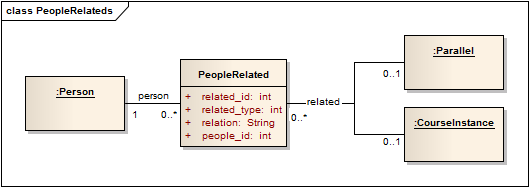
\includegraphics[width=12cm]{figures/PeopleRelateds}
\caption{Dekompozice pomocí polymorfní asociace}
\label{fig:polymorfni}
\end{center}
\end{figure}

\begin{table}[h]
\begin{center}
\begin{tabular}{|l|c|l|}

\hline
\textbf{Atribut} & \textbf{Příklad} & \textbf{Popis} \\ \hline
related\_id & 1 & cizí klíč záznamu, který je v asociaci s osobou \\\hline
related\_type & Parallel & jméno modelu ke kterému patří cizí klíč \\ & & v attributu \textit{related\_id} \\ \hline
relation & teachers & název asociace \\\hline
people\_id & 100 & cizí klíč pro osobu  \\\hline

\end{tabular}
\caption{Popis atributů tabulky PeopleRelated}
\label{tab:people_related}
\end{center}
\end{table}


\subsubsection{Hodnotící formuláře}
Z důvodu možné změny hodnotících formulářů v budoucnosti, jsem vytvořil návrh, který umožní vytvářet nové typy formulářů, nebo upravovat již existující. Formuláře se definují šablonou. Tato šablona definuje základní vlastnosti: minimální, maximální počet vyplnění, název a kdo může formulář vyplnit. Samotný obsah šablony formuláře se skládá z položek. Položky formuláře mohou být hodnotící tabulka, nadpis, hodnocení, text a jiné. Na obrázku \ref{fig:dynamicform} je doménový model dynamický formulářů.

\begin{figure}[h]
\begin{center}
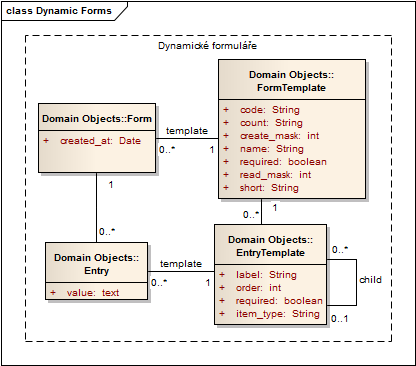
\includegraphics[scale=0.6]{figures/DynamicForms}
\caption{Doménový model dynamických formulářů}
\label{fig:dynamicform}
\end{center}
\end{figure}

Hodnotící formuláře se generují podle šablony formuláře získané z databáze. Šablona je reprezentovaná modelem \textit{FormTemplate}. Obsahuje veškeré informace potřebné pro formulaci chování formuláře. Mezi základní vlastnosti, které definuje šablona, patří název, popis a kód. Kód šablony je velmi důležitá vlastnost, definuje skupinu kam patří formulář. Skupiny formulářů jsou rozděleny podle druhu formuláře a ty popisuji v sekci hodnocení výuky \ref{sec:formulare}. Rozdělení formulářů do skupin s kombinací data vytvoření využívám pro verzování šablon. Šablony musím verzovat, jinak by mi při úpravě nebo smazání existující šablony, mohla nastat ztráta dat z vyplněných formulářů.

%Formuláře jsou rozděleny do skupin protože se časem mohou upravovat a nemůžu si dovolit upravit již vytvořenou šablonu. Mohlo by nastat ztráta dat ve vyplněných formulářích, proto se musí vždy vytvořit nová šablona.  

Šablona formuláře definuje také postupné hodnocení. Pro otevření dalšího formuláře se musí splnit několik podmínek:

\begin{enumerate}
\item Povinný formulář musí být vyplněn a také musí splnit podmínku pro minimální počet. V jiném případě není potřeba vyplnit žádný formulář.
\item Minimální počet lze definovat buď přesným počtem, nebo dynamicky podle asociace. Kde minimální počet mi definuje počet instancí v asociaci. Počet vytvořených formulářů se počítá pouze z jednoho hodnocení hospitace.
\item Hospitující i hospitovaný může vyplnit maximálně jeden formulář.
\end{enumerate}

U dynamických formulářů jsem musel také řešit jejich chování pro různé role v systému. Proto jsem přidal do šablony dva atributy s bitovými maskami rolí jedna maska pro role, které mohou zobrazit formuláře, druhá maska pro vyplnění formuláře. Používám stejný způsob rozlišování rolí v bitové masce jako u rolí pro uživatele viz \ref{sec:role}.

Obsah formuláře generuji pomocí položek, ty jsou reprezentovány modelem \textit{EntryTemplate}. Položky formuláře definují co se má vykreslit a kde. Umístění jednotlivých položek v dokumentu je definované ve stromové struktuře \ref{fig:tree_form}, kde kořenem stromu je šablona formuláře a ta se postupně větví přes potomky. Co se má vykreslit je definované atributem typu elementu. Seznam podporovaných typů elementů a jejich vlastnosti jsou vypsány v tabulce \ref{tab:elements}. Samotné generování obsahu není složitý proces. Celý formulář se sestaví hierarchicky i s hodnotami z modelu \textit{Entry}.

\begin{figure}[h]
\Tree [.FormTemplate [.EntryTemplate\\(ranking\_table) [.EntryTemplate\\(ranking) ][.EntryTemplate\\(ranking) ]] [.EntryTemplate\\(text) ] [.EntryTemplate\\(label) ]]

\caption{Příklad stromové struktury formuláře}
\label{fig:tree_form}
\end{figure}

Nestačí nám pouze vygenerovat formulář, ale potřebujeme i uložit jeho hodnoty do databáze. O to se starají modely \textit{Form} a \textit{Entry}. Model \textit{Form} složí pro identifikaci konkrétního vyplněného formuláře. Jednotlivé hodnoty z vyplněného formuláře jsou uložené v \textit{Entry} \ref{fig:data_form}.

\begin{figure}[h]
\Tree [.Form [.Entry\\(A) ] [.Entry\\(B) ] [.Entry\\(text) ]]
\caption{Příklad uložených dat}
\label{fig:data_form}
\end{figure}
%[.Entry [.B]] [.Entry [.text]]
\subsection{Výstup} 
Výstupem této iterace byla aplikace, která již využívala pouze svoji databázi pro zdroj dat z KOSu a dynamické formuláře s nadefinovanými šablonami formulářů. 

\section{Třetí iterace}
\subsection{Zadání}
Zadáním třetí iterace bylo připravit server pro službu FELid. Dalším požadavkem bylo zprovoznění automatického zálohování databáze.

\subsection{Postup}
\subsubsection{Nasazení aplikace}
Na diagramu nasazení \ref{fig:deployment} jsou znázorněny komponenty potřebné pro nasazení aplikace. Protože na serveru byl nainstalován pouze webový server Apache HTTP Server a databázový systém Mysql, bylo potřeba nainstalovat platformu Ruby a framework Ruby on Rail. K instalaci Ruby jsem se rozhodl použít software RVM. Instalaci jsem provedl podle návodu pro více uživatelskou instalaci \cite{RVM}. Tento program dovolí nainstalovat různé platformy Ruby na jednom počítači. Další přínosem je spravování gemsets\footnote{balíky knihoven mezi kterými lze přepínat pro různé aplikace}, díky nimž lze zprovoznit několik aplikací zároveň na jednom počítači. Do nainstalovaného webového serveru bylo potřeba ještě přidat zásuvný modul, který umožní nasadit Rails aplikace. Modul se jmenuje Passanger (mod\_rails) a instaloval jsem ho do Apache podle návodu na oficiálních stránkách \cite{passenger}.

\subsubsection{FELid}
Pro zprovoznění služby FELid, bylo potřeba splnit několik požadavků. Tyto požadavky jsou umístěny na oficiálních stránkách služby \cite{felid_pozadavky}. Jeden z požadavků je zprovoznění programu, který zajistí komunikaci se službou FELid. Tento program se jmenuje Shibboleth a obsahuje zásuvný modul mod\_shib do webového serveru. Při konfiguraci programu jsem postupoval podle návodu, který se nachází na wiki stránkách FELid \citep{felid}. Po splnění všech požadavků stačilo jen zažádat o registraci aplikace.

\begin{figure}[h]
\begin{center}
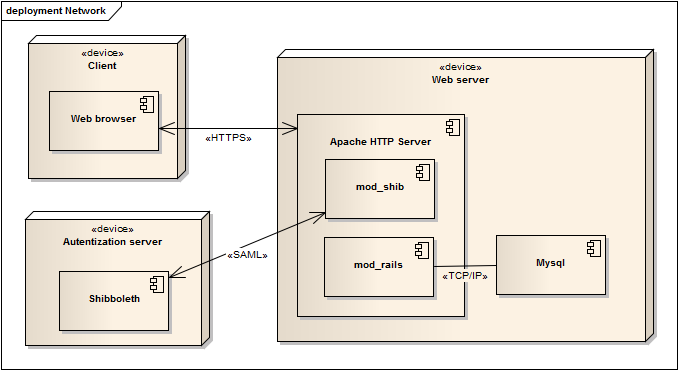
\includegraphics[width=12cm]{figures/deployment}
\caption{Diagram nasazení}
\label{fig:deployment}
\end{center}
\end{figure}

\subsubsection{Zálohavání databáze}
Pro automatické zálohování databáze jsem použil existující řešení  Ruby aplikace \textit{Backup} pro zálohování databází. Tato aplikace každý den vytvoří zálohu databáze, kterou uloží na disk. Na disku uchovává 300 záloh databáze, při překročení počtu záloh se starší zálohy nahrazují novými. Výhodou tohoto řešení je podpora různých databázových systémů a možnost ukládat zálohy na externí uložiště\footnote{pro příklad Amazon Simple Storage Service (S3)}. Záloha se spouští pravidelně pomocí programu \textit{Cron} každý den brzy ráno příkazem:
\begin{verbatim}
backup perform --trigger backup
\end{verbatim} 

\subsection{Výstup} 
V této iteraci se mi podařilo zprovoznit aplikaci na serveru a otestovat její funkčnost. Také jsem pracoval na programu, který jsem upravoval podle získaných připomínek od zadavatele z minulých iterací.

\section{Čtvrtá iterace}
\subsection{Zadání}
Tato iterace je poslední a proto většinu zadání tvořily připomínky od zadavatele. V této iteraci patří mezi hlavní úkoly vytvoření modulu, který bude generovat emailové zprávy po vyplnění hodnotícího formuláře a integrovat autentizaci přes FELid. 
\subsection{Postup}
\subsubsection{Autentizace}
V této fázi vývoje byla aplikace zaregistrována ve FELid. Před integrováním autentizace přes FELid, je potřeba otestovat aplikaci. Nejdůležitější je otestovat správnou funkčnost autorizace u všech rolí v celém systému. Po zprovoznění autentizace přes FELid není možné jednoduše testovat aplikaci pod různými uživateli. Od zprovoznění nebudu mít totiž kontrolu nad autentizací.

Integrace do aplikace je pak velmi jednoduchá. Stačilo jen odstranit dočasný způsob autentizace, který jsem implementoval v první iteraci. Aplikace FElid poskytuje aplikaci informace o přihlášeném uživateli prostřednictvím atributů v proměnné \verb|request.env|. Pro identifikaci přihlášeného uživatele používám atribut \verb|felid-uid| ve kterém se nachází uživatelské jméno. Autentizaci v aplikaci se stará jen jedna funkce \verb|current_user_session|.

\begin{quote}
\begin{verbatim}
def current_user_session
    return @user if defined?(@user)
    if not request.local? and not request.env["felid-uid"].nil? 
      and @user.nil? 
    then
      @user = People.find_by_username request.env["felid-uid"]
    end
    return @user
end
\end{verbatim} 
\end{quote}

\subsubsection{Emaily}
Jeden z požadavků bylo odesílání emailových zpráv po vyplnění hodnotícího formuláře. Součástí zadání je generování emailů ze šablon. Šablona se skládá z předmětu, textu zprávy a názvu akce. Akce v systému mohou být různých druhů, podle zadání stačilo pouze implementovat akce pro vytvoření formulářů. Při vykonání akce se vygeneruje emailová správa ze šablony emailu.

\subsubsection{Generátor obsahu emailových zpráv}
Protože je potřeba generovat do emailu proměnná data z hospitací, tak jsem vytvořil knihovnu \textit{EmailTemplates} pro generování obsahu emailů. Úkolem modulu je nahradit značky v textu za skutečná data. Pro vložení generovaných dat se používá zápis \verb|%značka%| do textu zprávy. 
\begin{quote}
Příklad vygenerování jednoduchého emailu se značkou pro kód předmětu.
\begin{verbatim}
text %course_code% => text A7B36ASS
\end{verbatim} 
\end{quote}

Při vývoji modulu jsem si dal za cíl vytvořit takovou knihovnu, která by umožnila jednoduše nastavit podporované značky. Největším zádrhelem v generování obsahu zprávy je získat data z hospitací. Protože vstupem do generátoru používám pouze instanci šablony a hodnocení hospitace, tak některá data musím získat přes několik relací mezi modely.

Knihovna obsahuje dva moduly. První částí je modul \textit{ModelHelper}, který slouží pro rozšíření libovolné třídy modelu v aplikaci. Rozšířenému modelu umožní pomocí statické metody \verb|attrs_tagged(*args)| povolit atributy ze kterých bude generátor získávat data. 

\begin{quote}
Příklad jednoduchého nastavení modelu \textit{Person}, které umožní generátoru vkládat jméno, emailovou adresu a uživatelské jméno.
\begin{verbatim}
class Person < ActiveRecord::Base
  include EmailTemplates::Tagged::ModelHelpers
    attrs_tagged :name, :email, :username
end
\end{verbatim} 
\end{quote}

Druhou částí je modul \textit{EmailBuilder}. Tento modul slouží pro vytvoření vlastního generátoru pomocí jednoduchého nastavování. Pro tyto účely modul poskytuje statickou metodu \verb|source(model,name,*path)|, ta slouží pro nastavení zdroje dat. Metoda dynamicky rozšíří třídu o metodu, ta dokáže získat data z aplikace. Využívá k tomu nastavení z modelu rozšířeného pomocí \textit{ModelHelper} a cesty k instancím modelu s daty. Cesta je definována posloupností názvů asociací mezi modely. 

\begin{quote}
Příklad implementace jednoduchého generátoru \textit{EmailBuilder}, který dokáže vkládat do emailů informace o hospitovaném učiteli. 
\begin{verbatim}
class EmailBuilder
  include Tagged::EmailBuilder
  source Person, :teacher, :evaluation, :teacher
end
\end{verbatim} 
Tento generátor bude podporovat tři značky \verb|%teacher_name%|, \verb|%teacher_email%| a \verb|%teacher_username%|. Tímto způsobem lze jednoduše nadefinovat velké množství značek.
\end{quote}

Struktura značky \ref{fig:znacka} se skládá ze dvou základních částí, ze jména zdroje a jména atributu, ze kterého generátor získá data pro nahrazení značky. 
\begin{figure}[h]
\Tree [.\%teacher\_name\% [.teacher (zdroj) ]  [.name (atribut) ] ]
\caption{Struktura značky}
\label{fig:znacka}
\end{figure}

Výhodou této knihovny je krátký a jednoduchý zápis pro vytvoření vlastního generátoru, který dokáže přes asociace mezi modely získávat data. V aplikaci jsem celkem nadefinoval pro devět zdrojů 32 značek.
 
\subsubsection{Odesílání emailů}
Dle zadání stačilo implementovat odesílání zpráv po vytvoření hodnotícího formuláře. Podle druhu hodnotícího formuláře se vygeneruje zpráva a odešle se administrátorovi hospitace, hospitujícím, hospitovaným garantovi předmětu a vedoucímu katedry. Do budoucna lze rozšířit v aplikaci odesílání emailů i při jiných akcí. Pro příklad se mohou odesílat při naplánování nové hospitace. 

Z časových a technických problémů se mi nepodařilo zprovoznit emailový server pro odesílání emailů, proto dočasně používám k odesílání emailový účet kvalitavyuky.gmail.com na Gmail.

\subsection{Výstup}
Výstupem z této iterace je finální aplikace, která splňuje všechny hlavní požadavky na funkčnost. 